\documentclass[a4paper,12pt]{article}
\usepackage{amsmath}
\usepackage[margin=0.9in]{geometry}
\usepackage{braket}
\usepackage{graphicx}
\begin{document}
\subsection*{Exercise 11.1}
For a fair coin $H(X)=-2\times\frac{1}{2}\log{\frac{1}{2}}=1$\\
For a fair die $H(X)=-6\times\frac{1}{6}\log{\frac{1}{6}}=1+\log{3}$\\
For an unfair coin we can write $H(X)=-p\log{p}-(1-p)\log{(1-p)}$ and 
for the unfair die $H(X)=-p_1\log{p_1}-p_2\log{p_2}-p_3\log{p_3}-p_4\log{p_4}-p_5\log{p_5}
-(1-p_1-p_2-p_3-p_4-p_5)\log{(1-p_1-p_2-p_3-p_4-p_5)}$.\\
Differentiating both of these we see that for both the global maxima is when 
all the probabilities are equal, therefore for the unfair coin and die the entropy will
decrease.
\subsection*{Exercise 11.2}
$I(p)=k\log{p}$ is a function of probability alone.\\
$\log{p}$ is smooth for $0<p\leq 1$\\
$I(pq)=k\log{(pq)}=k(\log{p}+\log{q})=I(p)+I(q)$
\subsection*{Exercise 11.3}
$H_{bin}(p)=-p\log{p}-(1-p)\log{(1-p)}$\\
$\displaystyle \frac{dH_{bin}}{dp}=-\frac{1}{\ln{2}}-\log{p}+\frac{1}{\ln{2}}+\log{(1-p)}=0$\\
$\displaystyle\frac{1-p}{p}=1$\\
Therefore, $p=\frac{1}{2}$.
\subsection*{Exercise 11.4}
For a function $f(x)$ to be concave we require $f^{\prime\prime}(x)<0$.\\
$\displaystyle \frac{d^2H_{bin}}{dp^2}=\frac{d}{dp}(\log{(1-p)}-\log{p})=
\frac{1}{\ln{2}(1-p)p}<0$\\
Hence, $H_{bin}$ is concave.
\subsection*{Exercise 11.5}
$H(p(x,y)||p(x)p(y))=\displaystyle\sum_{xy}p(x,y)\log{\frac{p(x,y)}{p(x)p(y)}}=
\sum_{xy}p(x,y)\log{p(x,y)}-\sum_{xy}p(x,y)\log{p(x)}-\sum_{xy}p(x,y)\log{p(y)}=
\sum_{xy}p(x,y)\log{p(x,y)}-\sum_{x}p(x)\log{p(x)}-\sum_{y}p(y)\log{p(y)}=
H(p(x))+H(p(y))-H(p(x,y))$\\
$H(p(x,y)||p(x)p(y))\geq 0$\\
Therefore,\\
$H(p(x))+H(p(y))-H(p(x,y))=H(X)+H(Y)-H(X,Y)\geq 0$\\
$H(X,Y)\leq H(X)+H(Y)$\\
If $X$ and $Y$ are independent then $p(x,y)=p(x)p(y)$. Therefore,\\
$H(X,Y)=-\displaystyle\sum_{xy}p(x,y)\log{p(x,y)}=
-\sum_{xy}p(x)p(y)\log{p(x)p(y)}=-\sum_{x}p(x)\log{p(x)}-\sum_{y}p(y)\log{p(y)}=H(X)+H(Y)$\\
Therefore, equality hold if and only if $X$ and $Y$ are independent.
\subsection*{Exercise 11.6}
$H(X,Y,Z)=-\displaystyle\sum_{xyz}p(x,y,z)\log{p(x,y,z)}=
-\sum_{xyz}p(x,y,z)\log{p(x|y,z)p(y,z)}=H(Y,Z)-\sum_{xyz}p(x,y,z)\log{p(x|y,z)}$\\
$H(X,Y)-H(Y)=H(X|Y)=-\displaystyle\sum_{xy}p(x,y)\log{p(x|y)}$\\
Then, using $\log{x}\leq (x-1)/\ln{2}$ we have,\\
$H(X,Y,Z)-H(Y,Z)-H(X,Y)+H(Y)=-\displaystyle\sum_{xyz}p(x,y,z)\log{p(x|y,z)}+\sum_{xyz}p(x,y,z)\log{p(x|y)}=
\sum_{xyz}p(x,y,z)\log{\frac{p(x|y)}{p(x|y,z)}}\leq \frac{1}{\ln{2}}\sum_{xyz}p(x,y,z)\left(
\frac{p(x|y)}{p(x|y,z)}-1\right)=\frac{1}{\ln{2}}\sum_{xyz}(p(x|y)p(y,z)-p(x,y,z))=
\frac{1}{\ln{2}}\left(\sum_{xy}p(x|y)p(y)-1\right)=
\frac{1}{\ln{2}}\left(\sum_{xy}p(x,y)-1\right)=\frac{1}{\ln{2}}(1-1)=0$\\
Hence,\\
$H(X,Y,Z)-H(Y,Z)\leq H(X,Y)-H(Y)$\\
with equality when $p(x|y,z)=p(x,y)$ which is the definition for a $Z\rightarrow Y\rightarrow X$
Markov chain.
\subsection*{Exercise 11.7}
$H(Y|X)=H(Y)-H(Y:X)=-\displaystyle\sum_yp(y)\log{p(y)}-
\sum_{xy}p(x,y)\log{\frac{p(x,y)}{p(x)p(y)}}=
-\sum_{xy}p(x,y)\log{p(y)}-\sum_{xy}p(x,y)\log{\frac{p(x,y)}{p(x)p(y)}}
=\sum_{xy}p(x,y)\log{\frac{p(x,y)}{p(x)}}=-H(p(x,y)||p(x))\geq 0$\\
Equality when $p(x,y)=p(x)$, therefore when $Y$ is a function of $X$, $Y=f(X)$.
\subsection*{Exercise 11.8}
For $p(x,y,z)$ we have
$p(0,0,0)=p(0,1,1)=p(1,0,1)=p(1,1,0)=\frac{1}{4}$ and $0$ otherwise. Hence,\\
$H(X,Y,Z)=-4\frac{1}{4}\log{\frac{1}{4}}=2$\\
$H(X,Y)=H(X,Z)=H(Y,Z)=-4\frac{1}{4}\log{\frac{1}{4}}=2$\\
$H(X)=H(Y)=H(Z)=-2\frac{1}{2}\log{\frac{1}{2}}=1$\\
Therefore,\\
$H(X,Y:Z)=H(X,Y)+H(Z)-H(X,Y,Z)=1$\\
$H(X:Z)=H(Y:Z)=H(Y)+H(Z)-H(Y,Z)=0$
\subsection*{Exercise 11.9}
For $p(x_1,x_2,y_1,y_2)$ we have $p(0,0,0,0)=p(1,1,1,1)=1/2$ and $0$ otherwise. Hence,\\
$H(X_1,X_2,Y_1,Y_2)=H(X_1,X_2)=H(X_1,Y_1)=H(X_2,Y_2)=H(Y_1,Y_2)=H(X_1)=H(X_2)=H(Y_1)=H(Y_2)=
-2\frac{1}{2}\log{\frac{1}{2}}=1$\\
Therefore,\\
$H(X_1:Y_1)+H(X_2:Y_2)=2H(X_1:Y_1)=2(H(X_1)+H(Y_1)-H(X_1,Y_1))=2$\\
$H(X_1,X_2:Y_1,Y_2)=H(X_1,X_2)+H(Y_1,Y_2)-H(X_1,X_2,Y_1,Y_2)=1$
\subsection*{Exercise 11.10}
If $X\rightarrow Y\rightarrow Z$ is a Markov chain then,\\
$p(Z|Y,X)=p(Z|Y)$\\
Using $p(X|Y)=\frac{p(X,Y)}{p(Y)}$ on both sides,\\
$\displaystyle\frac{p(Z,Y,X)}{p(Y,X)}=\frac{p(Z,Y)}{p(Y)}$\\
$\displaystyle\frac{p(Z,Y,X)}{p(Z,Y)}=\frac{p(Y,X)}{p(Y)}$\\
$p(X|Y,Z)=p(X|Y)$\\
Therefore, $Z\rightarrow Y\rightarrow X$ is also a Markov chain.
\subsection*{Exercise 11.11}
$\rho=\begin{bmatrix}
    1&0\\
    0&0
\end{bmatrix}\\
S(\rho)=-1\log{1}=0$\\
$\rho=\frac{1}{2}\begin{bmatrix}
    1&1\\
    1&1
\end{bmatrix}\\
\lambda= 1$ or $0$\\
$S(\rho)=-1\log{1}=0$\\
$\rho=\frac{1}{3}\begin{bmatrix}
    2&1\\
    1&1
\end{bmatrix}\\
\lambda= \frac{1}{2}\pm\frac{\sqrt{5}}{6}$\\
$S(\rho)=-(\frac{1}{2}+\frac{\sqrt{5}}{6})\log{(\frac{1}{2}+\frac{\sqrt{5}}{6})}
-(\frac{1}{2}-\frac{\sqrt{5}}{6})\log{(\frac{1}{2}-\frac{\sqrt{5}}{6})}\approx 0.55$\\
\subsection*{Exercise 11.12}
$\rho=\frac{1}{2}\begin{bmatrix}
    1+p&1-p\\
    1-p&1-p
\end{bmatrix}$\\
$\lambda = \frac{1}{2}\pm\frac{1}{2}\sqrt{1-2p(1-p)}$\\
$S(\rho)=-\frac{1}{2}((1+\sqrt{1-2p(1-p)})\log{\frac{1}{2}(1+\sqrt{1-2p(1-p)})}\\
+(1-\sqrt{1-2p(1-p)})\log{\frac{1}{2}(1-\sqrt{1-2p(1-p)})})$\\
$H(p,1-p)=-p\log{p}-(1-p)\log{(1-p)}$\\
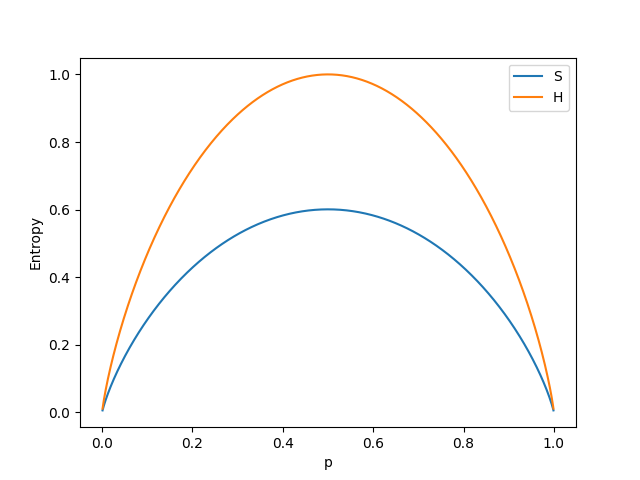
\includegraphics[scale=0.5]{12.png}\\
Therefore, $S(\rho)\leq H(p,1-p)$.
\subsection*{Exercise 11.13}
First note that for $\rho=\displaystyle\sum_i p_i\ket{i}\bra{i}$, 
$H(p_i)=\displaystyle -\sum_ip_i\log{p_i}=S(\rho)$. Then using the joint entropy
theorem for $\rho_i=\sigma$ $\forall i$ we have,\\
$S(\rho\otimes \sigma)=S(\displaystyle\sum_ip_i\rho\ket{i}\bra{i}\otimes \sigma)=
H(p_i)+\sum_ip_iS(\sigma)=S(\rho)+S(\sigma)$\\
Otherwise from the definition of the entropy for 
$\rho=\displaystyle\sum_i p_i\ket{i}\bra{i}$ and
$\sigma=\displaystyle\sum_j q_i\ket{j}\bra{j}$ we have,\\
$S(\rho\otimes \sigma)=S\left(\displaystyle\sum_{ij}p_iq_j\ket{i}\ket{j}\bra{i}\bra{j}\right)=
-\sum_{ij}p_iq_j\log{p_iq_j}=-\sum_ip_i\log{p_i}-\sum_jq_j\log{q_j}=S(\rho)+S(\sigma)$
\subsection*{Exercise 11.14}
If $\ket{AB}$ is a pure state of the composite system then $\ket{A}$ is a pure state
if and only if there's no entanglement. Hence, $S(A)\neq 0$ if and only if $\ket{AB}$ is
entangled. As $\ket{AB}$ is a pure state $S(A,B)=0$, and therefore
$S(B|A)=-S(A)$. As $S(A)\geq 0$, $S(B|A)<0$ if and only if $\ket{AB}$ is entangled.
\subsection*{Exercise 11.15}
\subsection*{Exercise 11.16}
\subsection*{Exercise 11.17}
\subsection*{Exercise 11.18}
\subsection*{Exercise 11.19}
\subsection*{Exercise 11.20}
\subsection*{Exercise 11.21}
\subsection*{Exercise 11.22}
\subsection*{Exercise 11.23}
\subsection*{Exercise 11.24}
\subsection*{Exercise 11.25}
\subsection*{Exercise 11.26}
\end{document}